\documentclass{report}

\usepackage[utf8]{inputenc}
\usepackage{titling}
\usepackage{natbib}
\usepackage{graphicx}
\usepackage{enumitem}
\usepackage{hyperref}
\usepackage{color}

%\usepackage[parfill]{parskip}

% Destroy the Annoying Margins.
\hoffset 0pt
\voffset 0pt
\headsep 0pt
\headheight 0pt
\oddsidemargin 0in 
\evensidemargin 0in 
\textwidth 6.5in \textheight 9in

\title{Cryptography}

\begin{document}

\begin{titlepage}
    \vspace*{-2cm}
    \begin{center}
        {\Huge \bfseries CST Training \par}
        \vspace{1cm}
        {\large \bfseries Cryptography  \par}

    \end{center}
    \begin{center}
        \vspace{3cm}
        
\includegraphics[scale=.6]{usna-seal.png}
        \vspace{1cm}
    \end{center}
    

  
    \begin{center}
        {\LARGE\bfseries United States Naval Academy \break \par}
        {\Large\bfseries Cyber Security Team \par}

    \end{center}
  
    \vspace{3.0cm}
   


\end{titlepage}


\newpage

\tableofcontents

\newpage

\chapter{Lesson Plan}
 
\section{Introduction}
This lesson will go in depth into the Ideas of Cryptography as it pertains to CTFs.
 
\section{Objectives}
 \begin{enumerate}
    \item Understand the language of Cryptography
    \item Understand where to start a Cryptography problem
    \item Understand the mathematical concepts that go into basic crypto 
    \item Recognizing classic crypto
    \item RSA
    \item AES and their modes
\end{enumerate}

\section{Credit}
Most of the information in this lesson plan was taken from Dr. George Nakos's SM350 Crypto and Information Security notes which can be found in the Google Drive.  And some comes from SI335 Algorithm notes authored by Dan Roche, with very occasional modifications by Chris Brown.

\newpage

\chapter{What is Crypto?}

\section{Definitions}
Many words in cryptology have multiple definitions, below are the technical definitions of some of those words, however you will still need some context to know what is being discussed.
\subsection{Crypto Words}
\begin{enumerate}
\item \color{blue}Cipher \color{black} or \color{blue}Cryptosystem \color{black} - method of secret communication between members of a group\newline
\item \color{blue}Plaintext \color{black} - A message before encryption\newline
\item \color{blue}Ciphertext \color{black} - An encrypted message\newline
\item \color{blue}Key \color{black} - is a set rules used to encrypt, or decrypt a message\newline
\end{enumerate}

\section{Types of Ciphers}
\subsection{Block Cipher}
A \color{blue}Block Cipher \color{black} is one where the plaintext is divided into blocks of fixed length and each block is encrypted in essentially the same way by using the same key.\newline
\newline
\subsection{Stream Cipher}
A \color{blue}stream cipher \color{black} is one where the plaintext is combined in some fashion with some pseudo-random character stream. This character stream may depend on previously encrypted text. The encryption is performed one character at a time and transformations of successive characters may vary.


\section{Types of Attacks}
The first step to any crypto problem is to figure out what cryptosystem is being used. After that, you can begin to figure out how to go about attacking it.

\subsection{Known Plaintext}
The attacker possesses some plaintext and its corresponding ciphertext. One may imagine that the plaintext and its corresponding ciphertext were somehow intercepted. The goal is to find the decryption key or more plaintext.

\subsection{Ciphertext Only}
Only some ciphertext is available to the attacker. The immediate goal is the decryption of the ciphertext. A further goal is to find the decryption key. This is the hardest type of attack.\newline \newline

\subsection{Chosen Plaintext}
The attacker can choose from several plaintexts and obtain their corresponding ciphertexts. One may think that the attacker possesses (at least temporarily) an “encryption machine” and he or she can encrypt any message. However, no key is available. The goal is to find the decryption key.
\newline \newline 
This is also a common CTF problem type where you connect to some server and they give you ciphertext and allow you to encrypt any plaintext you want.
\newline \newline For these, they roll their own crypto so you will not know what they cryptosystem is
\newline \newline The technique for this one is to figure out how certain things map or the ciphertext.  (ex. Are ‘A’s always mapped to ‘Q’s? If ‘A’ maps to ‘Q’ does ‘AA’ map to ‘QQ’?) A good step 1 is to enter the alphabet and see what it returns.
\newline

\section{CTFs}
\color{blue}Ciphertext only \color{black}  and \color{blue}known plaintext \color{black} are two of the most common types of crypto problems that you will encounter.  Ciphertext only is the hardest attack to perform and is always inadvisable unless there is no better option.  
With some ingenuity, creativity, and just a little bit of luck we can sometimes turn a Ciphertext only into a known Plaintext attack.  
To do this you have to think about: 
what has to be in the ciphertext?  
Note there isn't one answer to this.  Some CTFs all have flags that start with ``flag\{'' or something like that.
This does not always work and sometimes have to resort to other Ciphertext only methods.

\vspace{1cm}
\section{References}
\label{ref:2}
\begin{enumerate}[label=(\alph*)]
\item George Nakos: \textit{Notes in Cryptology} \url{ https://drive.google.com/open?id=1-naxKPbzHIjCFrDy5nYSHtKKW3LiIJ4j}
\end{enumerate}

\chapter{MATHE}
\section{Notation}
In Order to fully understand how most cryptosystems work we will talk about them in some degree of mathematical notation and referencing certain mathematical operations that may not be familiar to you.\newline 
\begin{itemize}
\item $ Z = \{0, \pm1, \pm2,...\} $ is the set of integers
\item $Z_n= \{0, 1, 2, ... n-1\}$ is the set of integers up to n
\item $Z^*_n$ is the set of invertibles modulo n $\rightarrow$ We will get to this.
\end{itemize}

\section{Modulus}
\subsection{Definition of Modulus}
Suppose \textit{a} is a non-negative integer, and \textit{m} is a positive integer. To both mathematicians and grade school students dividing 
$a$  by $m$ means there are two numbers, a quotient $q$ and a remainder $r$, 
such that $a=qm+r$, where $0 \leq r<m$. In fact, $q$ and $r$ are unique. The definition of ``$a$ mod $m$" is such that it equals the remainder $r$.

As we will see, this operation of ``mod" actually defines a separate world of calculation, for each different denominator (or ``modulus") $m$. By this I mean, if we do all of our normal arithmetic operations ``mod $m$", then some interesting patterns emerge.

\subsection{Modular Addition}
Let's look at the ``world" that gets created with the operation of addition and the modulus \(m=15\). Figure 3.1 shows \(a+b\bmod 15\) for every \(a,b\) from 0 up to 14.

\begin{figure}[!ht]
  \centering
  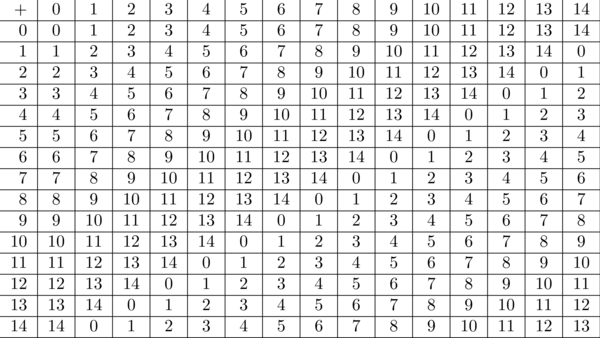
\includegraphics[width=85mm,scale=0.5]{s15.png}
  \caption{Addition mod 15}
\end{figure}


What if we added up bigger numbers and took the sum mod 15? As it turns out, that is exactly the same as if we took the big integers mod 15 first, then took their sum mod 15. Since every ``mod 15" gives an integer in the range above (0 to 14), that's really all there is.
\newline
\newline
In case that last paragraph lost you, here's a formal restatement:

Theorem

For any integers \(a,b,m\) with \(m > 0\),

\((a + b) \bmod m = (a \bmod m) + (b \bmod m) \bmod m\)

\subsection{Subtraction}

Subtraction is just like addition, with a negative number. So \(24 - 11\) is really just \(24 + (-11)\). And a negative number is just something that adds with the original number to zero. For example, -11 is just the number that, when added to 11, gives us 0.

No surprises so far. But let's try to apply these concepts to the ``mod 15" world. 
Look back at the table and you'll see that a single 0 appears in every row and column. 
This corresponds to the additive inverse mod 15! In fact, we can say exactly what it is: For any \(1\leq a < m\), \(-a\bmod m\) is equal to \(m-a\). This makes sense, because \(a+(m-a)=m\), which is always equal to 0 mod m.

So this means that we can write things like \(4 - 10 \bmod 15\), and it makes sense. And since subtraction is just a short-hand for addition, the same rule as above applies: we can take \(-10\bmod 15\) and add it to 4, or we can subtract \(4-10=-6\) and take that mod 15 — either way, it's always going to come out the same.

\subsection{Modular Multiplication}

Now let's delve into the world of multiplication mod 15:

\begin{figure}[h!]
  \centering
  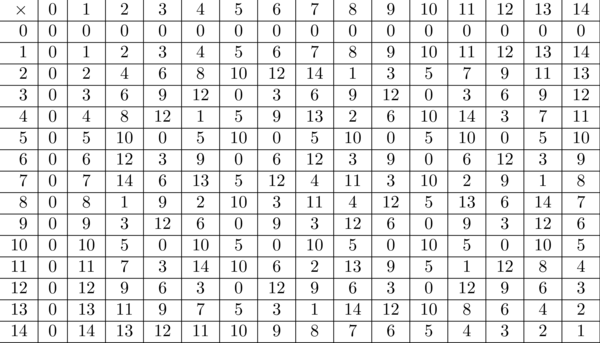
\includegraphics[width=90mm,scale=0.5]{m15.png}
  \caption{Multiplication mod 15}
\end{figure}


The first thing we need is another theorem analogous to the one above on taking ``mod"s before or after addition:


Theorem

For any integers \(a,b,m\) with \(m > 0\),

\((ab) \bmod m = (a \bmod m)(b \bmod m) \bmod m\)
\newline
\newline
So multiplying a and b, then taking the answer mod m, is the same as taking each of a and b mod m, then multiplying and doing one last mod m to get the same result, every time.

\subsection{Modular Division}
Sometimes called the Multiplicative Inverse. First, We need to recognize that division is really just multiplication with an inverse. So \(a/b\) just means \(a\times b^{-1}\), where \(b^{-1}\) is defined as the number which, when multiplied by $b$, gives 1.

So look up at the table for multiplication mod 15 to see if we can find some inverses. We're looking for a ``1" in every row and column...

Some numbers have a multiplicative inverse. Like \(13\times 7 \bmod 15= 91\bmod 15 = 1\), so \(13^{-1} \bmod 15 = 7\). This means we can do division by 13 (or by 7) in the ``mod-15 world".

But some of the numbers don't have any inverse mod 15. Specifically, 0, 3, 5, 6, 9, 10, and 12 have no ``1" in their rows or columns, hence no multiplicative inverse. If you think for a minute, you might realize that these are exactly the numbers that share a common factor with 15.

\vspace{1cm}
\section{References}
\label{ref:3}
\begin{enumerate}[label=(\alph*)]
\item George Nakos: \textit{Notes in Cryptology} \url{https://drive.google.com/open?id=1-naxKPbzHIjCFrDy5nYSHtKKW3LiIJ4j}
\item USNA SI335 Algorithms: \textit{Modular Arithmetic} \url{https://www.usna.edu/Users/cs/wcbrown/courses/S18SI335/notes/03/notes.html#3}
\end{enumerate}

\chapter{Basic Ciphers}
The first step of any crypto problem is figuring out what type of cryptosystem you are working with.
\section{Shift Cipher}
The \color{blue} Shift Cipher \color{black} is perhaps the simplest and certainly one of the oldest ciphers. We encrypt a message by replacing each letter with the letter obtained by a fixed amount of shifting. The shifting wraps around if it has passed the end of the alphabet.  
\newline
Now we may define the Shift Cipher, mathematically. If our alphabet consists of the 26 characters a,b,...,z, we convert each letter of our message into a corresponding integer from 0 to 25 using the natural orders: a -\(>\) 0, b -\(>\) 1, … z -\(>\) 25.  
\subsection{Caesar Shift}
A cipher that shifts the same number of letters for each letter of the plaintext is known as the \color{blue} Caesar Shift \color{black} it is named after Julius Caesar.  It is a block cipher of length 1.\newline \newline 

Encryption(x) \(= a + b \bmod n \)

Where \(a\) is the numerical value of the letter being shifted and \(b\) is the number of spots to shift and \(n\) is the size of the alphabet 
\newline
\newline
Traditionally these ciphers are used in mod 26.  The way to encrypt/decrypt these is to turn the text into the corresponding numbers and shift over the key and mod 26.
*Note: It is not uncommon for a CTF to not have a modulus and may shift everything over by some larger number that may place the unicode value outside of English characters. However, we’re clever and we know the most commonly used character in English and can usually guess what the shift is based on statistical analysis. (hint it is:  )
\subsection{Affine Cipher}
This is another shift cipher similar to the Caesar Shift but it enlarges the key space by multiplying as well as adding to the value of the current letter. \newline \newline

Encryption(x) \(= (a\times x + b) \bmod n\)

for some key (a, b), with $a, b \in Z_n$.  To decrypt you merely reverse the function.

Decryption(y) = $a^{-1}*(y - b) \bmod n$

Where a-1 is the multiplicative inverse of $a \bmod 26$.\newline
Recall that a is invertible in $Z_26$ if and only if gcd (a, 26) = 1.

\subsection{The Vigenère Cipher}
Encryption with the \color{blue} Vigenere Cipher \color{black} is done as follows: We pick a keyword of length, say, m. We divide the plaintext into blocks of size m. Then to each block we “add” the keyword by switching to numbers and adding modulo n, where n is the size of the alphabet. If the length of the plaintext is not a multiple of m, then we add random text so that the length becomes a multiple of m.  Is a block cipher of size m.

\section{The Perfect Cipher: The One-Time Pad}
The \color{blue} One-Time Pad \color{black} or \color{blue} Vernam Cipher \color{black} is the 
special case of Vigenere Cipher where the plaintext length is equal to the key-length.  So, 
there is only one block of encryption


The One-Time Pad is very secure. It is used for top secrets and for arming or disarming nuclear
weapons. However, it is not easy to use, because the keys are as large as the message itself. 
Each key can only be used once. Then it should be discarded. If the key is re-used, then this 
process can be viewed as an ordinary Vigenere Cipher with repeated keyword and it becomes 
vulnerable to the usual attacks.

It is considered perfectly secure such that no matter how smart someone is or how fast their
computer is, they will never be able to crack it without the key.  This is due to the fact 
that there can be multiple plaintexts for one ciphertext.  For example, if you wanted to 
encrpyt ``Attack at Dawn'' you take a key that is as long as your plaintext (14) such as 
a key (in hex bytes): a38c4f05297c27587113c6b252d1.  You use each byte of this key and xor it
with each byte of the plaintext and get the ciphertext: e2f83b644a170739053382d325bf.  There 
exists a key such that this same cipher text decrypts to ``Make peace now''.  Therefore, without
the key it is impossible to reverse the ciphertext to the plaintext. 

\section{Learning More}
George Nakos's Crypto Notes in the google drive $\rightarrow$ CST19 $\rightarrow$ Books 
$\rightarrow$ Crypto.  Is a great resource to learn more about Cryptology and to learn
about many different ciphers and hash functions.
\hyperref[ref:4]{\textbf{References: (a)}}

\vspace{1cm}
\section{References}
\label{ref:4}
\begin{enumerate}[label=(\alph*)]
\item George Nakos: \textit{Notes in Cryptology} \url{https://drive.google.com/open?id=1-naxKPbzHIjCFrDy5nYSHtKKW3LiIJ4j}
\end{enumerate}

\chapter{Other Topics}

\section{Encryption vs. Encoding}
\color{blue} Encoding \color{black} transforms data into another format using a scheme that is publicly available and does not require a key.  Encodings can easily be reversed. 

The purpose of \color{blue} encryption \color{black} is to transform data in order to
keep it secret from others.  Encryption transforms data into another format in such a
way that only specific individual(s) can reverse the transformation. It uses a key, which
is kept secret, in conjunction with the plaintext and the algorithm, in order to perform 
the encryption operation. 

\subsection{Base64}
Base64 is an example of an encoding scheme.  Base64 is used quite a bit and therefore is something that you should know and be able to recognize on the spot.  To recognize it, look for the distinctive equal signs (``=") at the end which is for padding the length of the string.  Other than that generally any string that uses Uppercase, lowercase, numbers, forward slash (``/"), and/or plus signs (``+") can be assumed to be Base64 encoded.
Example: VGhpcyBpcyBhIEJhc2U2NCBlbmNvZGVkIHN0cmluZw==
To decode, google Base64 decoder or just go to \url{https://www.base64decode.org/}

\hyperref[ref:5]{\textbf{References: (a)}}

\section{XOR}
XOR is a bitwise operator in which you compare to bits and if they are the same, the result is a zero and if they are different the result is a one.  Example:


     				$0101 \oplus 0011  = 0110$
                                 
XORing is a common function that is used in most encryption schemes.
To do any problem that might have been xor-ed download \color{blue} \href{https://github.com/hellman/xortool}{xortool} \color{black} and install it.
This program is great for brute forcing something that has been xor-ed with an 
unknown key.  It also has an xortool-xor program that xor’s things which can be handy.
\hyperref[ref:5]{\textbf{References: (b)}} 

ADD XOR SAMPLE PROBLEM

\section{Hashing Functions}
A hashing function is a function that is used to take arbitrarily large input and 
condense it down into a fixed length output.  A good hash function could be something
as simple as 
\[h(x) = \left(\left(ax + c\right) \bmod p\right) \bmod s \]
(where this is a Carter and Wegman Hash Function).  This formula will take in however 
much data and it will always return the same length output.  Another key factor of a 
hash function is that the output will always be the same for the same input.  

For a hash function to be secure, it must not be easy to generate a hash collision
(i.e. two inputs map to the same output).  Through the pigeon hole principal, we
know that since there is infinitely many different inputs and a fixed number of
outputs then there has to be collisions.  MD5 used to be a widely used hash function
but has since been broken due to being about to easily create collisions in it.  SHA1
has also been broken.  Currently SHA2, and SHA256 are some of the more common hash 
functions where it is still difficult to generate a collision which makes these 
considered secure.

\section{Resources}
There are some various online and downloadable tools and resources that are at your disposal.  Some of the ones that I have found useful over the years are:
\begin{itemize}
\item \url{https://quipqiup.com/} which is an online cryptogram solver.  This will solve a lot of your polymorphic and substitution ciphers.  It is usually my first stop when I do not know how the given ciphertext was encrypted.  
\item \href{https://github.com/nccgroup/featherduster}{https://github.com/nccgroup/featherduster} which is a github repository that will look scan some ciphertext and try to determine how it was encrypted and see if it can decrypt it.  
\item \url{http://www.factordb.com/} Factordb is a web database in which you can input a large number and it will tell you if it is prime or composite and if it is composite it will lookup in its database the prime factors of the given number.  
\item \url{https://www.alpertron.com.ar/ECM.HTM} Alpertron is a large number integer factorization calculator.  You input a number and it will start calculating the prime factors of it for you.  This calculator will find the prime numbers but depending on the number that you give it, it may take longer than you are willing to let it run.  This is a good resource to use because sometimes the vulnerability in the RSA problem that you are given is that the prime numbers were chosen poorly and this tool can help you find them.  That being said, if it runs for over about 10 hours, I would stop it and try a different approach. 
\item \href{https://github.com/ius/rsatool}{rsatool} rsatool is another github repository for a tool that helps you do most of the math used in calcuating the different variables when working with rsa.  This tool cannot break rsa but makes working with rsa easier.
\item \href{https://github.com/hellman/xortool}{xortool} As previously mentioned, xortool is a great resource to use for xor problems and it comes with another tool called xortool-xor which lets you easily xor two things together.
\end{itemize}

\vspace{1cm}
\section{References}
\label{ref:5}
\begin{enumerate}[label=(\alph*)]
\item Base64: \textit{Decoder/Encoder} \url{https://www.base64decode.org/}
\item github: \textit{hellman xortool} \url{https://github.com/hellman/xortool}
\end{enumerate}

\chapter{The RSA Cryptosystem}

\section{First Glance}
RSA is one of the two most common Crypto CTF problem that you will encounter.  There are a lot of different moving parts, a lot of varieties in what can be done, and there are a lot of things that can go wrong.  At a first glance it may seem extremely complicated and difficult to understand but we will try and break it down so that it is simple and easy to understand.

There are a lot of resources out there for RSA but one of the biggest and best is simply the Wikipedia page.  I have gone to the Wikipedia page countless times during many different CTFs looking for more information on RSA.  \hyperref[ref:6]{\textbf{References: (a)}}

\section{How Does It Work}
The security of this cryptosystem is based on the belief that it is computationally hard to factor large integers that are products of large primes.  It starts out by computing two large prime numbers $p$ and $q$.  Then there is a large semiprime (only two prime factors) number $n$ that is the multiplication of $p$ and $q$, $p \times q = n$. $n$ is a large number and by large we mean in the magnatude of 2048 bits which can be up to about 600 digits.  RSA, which is deeply dependent on modular arithmetic, uses this $n$ as its modulus.  We also need a number $\phi(n)$ which is simply calculated by $(p-1)\times(q-1) = \phi(n)$.  

So far all of this should be pretty straight forward and easy to understand.  Next comes the public exponent $e$.  $e$ is a number (usually either 3 or 65537) such that it is modularly invertible to $\phi(n)$.  All that this means is that gcd($e$, $\phi(n)$) = 1. So $e$ and $\phi(n)$ are coprime. This means that they are not prime in of themselves but they share no common factors except 1 (e.g. 9 and 10 are coprime).

Now for the private exponent, $d$.  $d$ is the modular inverse of $e \bmod \phi(n)$. Therefore $d = e^{-1} \bmod \phi(n)$ or more easily stated $d\times e = 1 \bmod \phi(n)$.  

In the end there are two keys, a public key and a private key.  The public key contains $e$ and $n$.  While the private key contains $p$, $q$, and $d$.

So to summarize:
\begin{itemize}
\item Let $p$ and $q$ be two primes and let $n = p \times q$.
\item Let $e$ be a positive integer which is invertible modulo $\phi(n) = (p - 1)(q - 1)$
\item Let $d = e^{-1} \bmod \phi(n)$.
\item The public key is $k_{pu} = (n, e)$.
\item The private key is $k_{pr} = (p, q, d)$.
\end{itemize}

\section{Encryption and Decryption}
\color{blue}Public Encryption \color{black}: A plaintext is first converted into an integer $x$ which is less than $n$. The encryption is done by using the public key (n, e) as follows where $y$ is an integer reprensentation of the ciphertext:
\[y = k_{pu}(x) = x^e \bmod n\]
\newline
\color{blue}Private Decryption \color{black}: The ciphertext $y$ is decrypted back to $x$ by using the secret number $d$ by the formula:
\[x = k_{pr}(y) = y^d \bmod n\]
\newline
rsatool can be used with $p$ and $q$ in order to find $d$.

\section{Elementary Attacks of RSA (given public key (n,e))}
\begin{itemize}
\item If $n$ is factorable: Plug n into \url{http://www.factordb.com/} or \url{https://www.alpertron.com.ar/ECM.HTM} and see if it finds anything.  If it can be factored then plug the factors into rsatool and get the $d$ and use that to decrypt the ciphertext
\item If $\phi(n)$ is known we can figure out $d$ as well as $p$ and $q$ which some basic math:   
		\[\phi(n) = (p - 1)(q - 1) \ \  \rightarrow \ \ \phi(n) = pq - (p + q) +  1 \ \ \rightarrow \ \  (p + q) = n - \phi(n) + 1\]
\item If the number of encrypted messages is equal to or greather than the exponent that is used.  This is usually seen with an exponent of 3. Use Chinese Remainder Theorm
\end{itemize}

\subsection{Chinese Remainder Theorm}
Let $a_1, a_2$ \textellipsis $a_k$ be any integers and let $m_1, m_2$ \textellipsis $m_k$ be distinct integers greater than 1 that are pairwise relatively prime. Then the systems of congruences:
\[x = a_1 \bmod m_1\]
\[x = a_2 \bmod m_2\]
\[...\]
\[...\]
\[x = a_k \bmod m_k\]

has a unique solution $x$. $x$ is given by formula:
\[x = (a_1 \times y_1\times M_1) + (a_2\times y_2\times M_2) + ... + (a_k\times y_k\times M_k) \bmod M\]
Where $M = m_1\times m_2\times ...m_k$,     $M_i= \frac{M}{m_i}$, and $y_i = M_i^{-1} \bmod m$
\newline In a CTF problem $x$ will be your plaintext and all the $a$'s will be all the ciphertexts.  It is to note that all the ciphertexts will be different but they will all decrypt to the same plaintext.

\section{RSA Small Exponent (little e) attack}
Public exponent of 3 used to be common because of quick encryption however if Alice wants to send the same message (x) to three different people and she uses three different n values (NOTE: This method applies to any case where the same message x is sent to k recipients by using the same exponent e = k.)
\[y_1=x^3 \bmod n_1\]
					\[y_2=x^3 \bmod n_2\]
					\[y_3=x^3 \bmod n_3\]
You can use the Chinese Remainder theorem to find $X \in Z_{n_1n_2n_3}$ such that:
					\[X=y_1 \bmod n_1\]
					\[X=y_2 \bmod n_2\]
					\[X=y_3 \bmod n_3\]

\chapter{AES (Advanced Encryption Standard)}
AES is a \color{blue} symmetric block cipher \color{black} that encrypts data in 128-bit blocks (16 bytes).  AES is generally the most used symmetric cipher and is one part of how most SSL connections are secured.

There are two main types (or modes) of AES: ECB (Electronic Codebook) and CBC (Cipher Block Chaining).

The internal intricacies on how AES works are not that important for the scope of most CTF problems.  But understanding how each produces their respective ciphertexts is.
NOTE: The internal intricacies on how AES encrypts stuff is discussed further under more of George Nakos' notes. \hyperref[ref:6]{\textbf{References: (b)}}

\section{ECB (Electronic Codebook)}
ECB is far less secure than CBC because ECB lacks \color{blue} diffusion\color{black}.  i.e. Each block is unaffected by other blocks.
\begin{figure}[h!]
  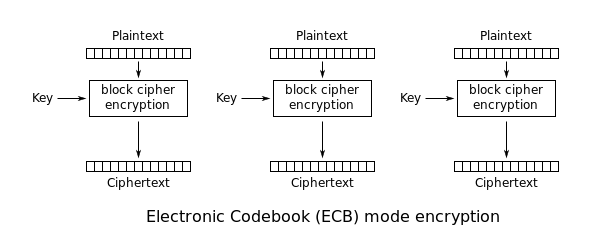
\includegraphics[width=\linewidth]{ECB_Walkthrough_.png}
\end{figure}

The reason why ECB mode of any block cipher is bad is that the same input always encrypts to the same output. The input is broken into fixed-length blocks and encrypted, and all of the blocks of identical input will create similarly equal output blocks. The data is all encrypted, but we know where their plaintexts were the same. 

There is no key recovery attack against this issue, at least not that I am aware of, but the problem is that the plaintext can be guessed.

Here is an example of a write-up of a CTF Crypto challenge that used ECB encryption
\href{https://michael-myers.github.io/blog/post/enigma2017-broken-encryption-writeup/}{Example}.  I highly suggest that you read through this write-up as it well written and can give a good insight into how bad ECB encryption is.

To reiterate what something that Mike talked about in his write-up: There are two main types of attacks against AES ECB encryption:
\begin{enumerate}
\item Given enough encrypted blocks and some partial knowledge of the plaintext (known offsets of fixed data, like as defined by filetype formats or communication protocols), statistical and frequency analysis (and some guessing, then confirming) can reveal partial plaintext.
\item Given the ability to prefix or circumfix (insert in the middle somewhere) arbitrary plaintext, and then have it encrypted and view the resulting ciphertext, an attacker can stage a Chosen Plaintext Attack.  (***MOST COMMON FOR CTFs***)
\end{enumerate}

\subsection{CTF examples}



\section{CBC (Cipher Block Chaining)}
CBC creates diffusion by XORing each plaintext with the ciphertext from the block before.  It also requires an IV (Initialization Vector) to XOR with the first plaintext.
\begin{figure}[h!]
  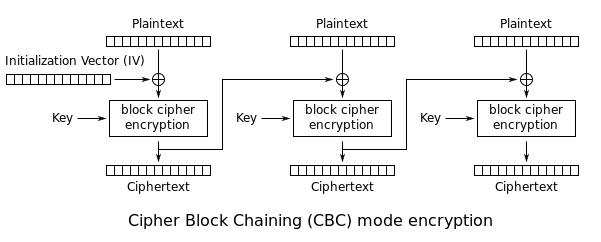
\includegraphics[width=\linewidth]{CBC_Walkthrough_.png}
\end{figure}

While not as vulnerable as ECB, AES CBC can have its weak points too.  To get a better understanding of how a CTF problem might use AES CBC I suggest that you read this \href{https://github.com/RandomsCTF/write-ups/tree/master/Defcamp\%20CTF\%20Qualification\%202015/No\%20Crypto\%20\%5Bcrypto\%5D\%20(200)}{write-up}.

\section{CTF problems}

\section{Other AES modes}

\chapter{Other Symmetric Cipher}
DES - Broken \newline
Triple DES (3DES) - arguably just as secure as AES but takes more computational power \newline
RC4 - Broken (How WEP and WPA was broken) You can read more about that in this \href{http://cr.yp.to/streamciphers/rc4biases-20130708.pdf}{paper}.
\newline \newline
None of these are really very important to learn but they will show up in CTFs from time to time so keep in mind that you may not always get an encryption method that you know about but if you can recognize it, then you can probably lookup how it has been broken in the past.

\section{Scripted Ciphers}
It is very common that for a Crypto challenge you will simply be given a netcat connection and port to connect to and sometimes even the code that that netcat connect is running on.  When this happens it is usually some python script where they implement some for of Cryptography (it can be RSA, AES, or something different entirely) and you have to figure out what they did wrong in order to decrypt their cipher.  




\vspace{1cm}
\section{References}
\label{ref:6}
\begin{enumerate}[label=(\alph*)]
\item Wikipedia: \textit{RSA} \url{https://www.wikipedia.org/wiki/RSA_(cryptosystem)}
\item George Nakos: \textit{AES \url{https://drive.google.com/open?id=1oEEcxZv33sPB2AHwBxbuBh9xvhHyAbnb}}
\end{enumerate}

\end{document}
